\documentclass[12pt]{article}

\usepackage{graphicx}
\usepackage{geometry}
\usepackage{setspace}
\usepackage{multirow}
\usepackage[table,xcdraw]{xcolor}
\usepackage{caption}
\usepackage{tocbibind} %Index of table of contents
\usepackage{url} 

\geometry{a4paper, total={170mm, 257mm}, left=20mm, right=20mm, top=25mm, bottom=25mm}
\usepackage[spanish,es-tabla]{babel}
\usepackage{fancyhdr}
\pagestyle{fancy}
\fancyhf{} % Limpia los estilos anteriores de encabezado y pie de página

\rhead{Tecnológico de Costa Rica}
\cfoot{\thepage} % Número de página en el centro
\renewcommand{\headrulewidth}{0.5pt}
\setlength{\parindent}{1em}
\setlength{\parskip}{1em}
\usepackage{makeidx}
\makeindex
%%%%%%%%%%%%%%%%%%%%%%%%%%%%%%%%%%%%%%%%%%%%%%%%%%%%%%%%%%%%%%%%%%%%%%%%%%%%%%%%%%%%%%%%%%%%%%%%%%%%%%%%%%%%%%%%%%%%%% here Begins the document

\begin{document}
\begin{titlepage}

  \centering
  \vspace{10cm}
  \textbf{\LARGE Instituto Tecnológico de Costa Rica}
  \vspace{2cm}
  \textbf{\LARGE Escuela de Ingeniería Electrónica}
  \vspace{2cm}
  
\includegraphics[width=10cm]{logotec/image.png}
  \vspace{2cm}
  \hrule
  \vspace{1cm}
  \textbf{\LARGE Desarrollo de un conjunto de flujos de trabajo para la implementación de software a bordo de computadoras de guía, navegación y control espacial (GNC)}
  \vspace{1cm}
  \hrule
  \vspace{1cm}
  \textbf{\LARGE SETECLab-TEC\\}
  \vspace{1cm}
  \textbf{\LARGE David Felipe Duarte Sánchez\\}
  \vspace{1cm}
  \textbf{\LARGE 2017239606}

  \vspace{1cm}
  \today % Esto agrega la fecha actual
\end{titlepage}
.
\par
\vspace{16cm} % Ajusta la cantidad de espacio vertical según sea necesario

Yo, David Felipe Duarte Sánchez portador de la cédula 305070982, declaro que los resultados obtenidos en el presente trabajo de investigación, previo a la obtención del título de licenciado en Ingeniería Electrónica, son absolutamente originales, auténticos y personales.

Soy consciente de que el hecho de no respetar los derechos de autor y realizar una mala conducta científica, es decir, fabricación de datos falsos y plagio, conlleva sanciones universitarias y/o legales.

En tal virtud, declaro que el trabajo de investigación realizado sujeto a evaluación no ha sido presentado anteriormente para obtener algún grado académico o título, ni ha sido publicado en sitio alguno y los efectos legales y académicos que se pueden derivar del trabajo propuesto de investigación son y serán de mi sola y exclusiva responsabilidad legal y académica.

\newpage
\tableofcontents
\newpage

\section{Entorno del proyecto}
El Tecnológico de Costa Rica es una institución de educación superior la cual contribuye al desarrollo integral del país, mediante la formación de recursos humanos, la investigación y la extensión, manteniendo el liderazgo científico, tecnológico y el estricto apego a las normas éticas, humanísticas y ambientales. En esta institución se imparte la carrera de Ingeniería Electrónica, encargada de formar profesionales de excelencia encargados de mejorar la calidad de vida mediante el uso racional del conocimiento de la electrónica \cite{conare_itcr_mision}.

Como parte de esta escuela se encuentra el laboratorio de sistemas espaciales SETEC-Lab, el cual es el encargado de velar por el aprovechamiento de las capacidades que ya tiene el Tecnológico de Costa Rica como institución y utilizarlas en el desarrollo de proyectos espaciales, promoviendo esta área como herramienta de desarrollo en el país. El SETEC-Lab tiene cuatro líneas de investigación \cite{tec_setec_lab}. 

La primera línea de investigación se relaciona con los algoritmos de operación de los sistemas de Guía Navegación y Control (GNC), los cuales se encargan de gestionar y optimizar el movimiento de aeronaves y vehículos autónomos, para comprender de una mejor forma el funcionamiento de estos algoritmos, a continuación, se explicará de que se encargan los segmentos de guía, navegación y control \cite{moghaddam2021guidance}. 

Por un lado, los algoritmos de guía determinan la trayectoria que se debe de seguir para alcanzar un destino específico, se debe de calcular la ruta más eficiente y además de esto se deben de tomar en cuenta factores como obstáculos, condiciones meteorológicas y restricciones de espacio aéreo. 

Por otro lado, el segmento de navegación se refiere a la capacidad del sistema de para poder determinar la posición actual y poder orientarse en el espacio. Estos utilizan datos de sensores como lo pueden ser sistemas de posicionamiento global (GPS) y Unidades de medida Inercial (IMU) con el fin de poder asegurar que siempre se mantenga la ruta planificada \cite{Colmenarejo2024}. 

Finalmente, los algoritmos de control son los encargados de ajustar los sistemas de propulsión y dirección del vehículo para mantener el curso deseado y así poder responder a las perturbaciones externas. Generalmente se pueden encontrar controladores adaptativos y sistemas de realimentación los cuales ajustan continuamente el comportamiento del vehículo para minimizar los errores y así garantizar la estabilidad \cite{Balaram2008}.
 
La segunda línea de investigación se encuentra relacionada con los sistemas de software para los sistemas GNC, esta área es la encargada de generar contenido como herramientas, métodos y artefactos para poder embeber de manera exitosa en el software requerido todos los programas y dependencias para que todos los módulos funcionen correctamente.

La tercera línea de investigación se encarga de los sistemas de potencia, esto con el fin de garantizar el funcionamiento seguro de los distintos componentes eléctricos. Estos sistemas incluyen múltiples fuentes de energía y tecnologías para garantizar el suministro eléctrico libre de interrupciones.

Finalmente, la cuarta área se encuentra sujeta al área de ingeniera de sistemas y diseño de misiones, esta área es la encargada de determinar los objetivos de la misión, planificación y gestión de riesgos y coordinar las múltiples áreas del proyecto con el objetivo de asegurar que todos los aspectos del proyecto se integren de forma efectiva \cite{Balaram2008}.


El SETEC-Lab es reconocido por haber desarrollado proyectos aeroespaciales como lo son el proyecto Irazú y el proyecto MUSA. Por un lado, el proyecto Irazú surge como una colaboración entre profesionales de la Asociación Centroamericana de Aeronáutica del Espacio (ACAE) y del Tecnológico de Costa Rica (TEC) con el objetivo de desarrollar las capacidades para llevar a cabo misiones espaciales, siendo una prueba de concepto de una plataforma con tecnología CubeSat para el monitoreo y cambio climático mediante la transmisión de datos de crecimiento forestal, variables ambientales y secuestro de carbono en los bosques tropicales de Costa Rica \cite{TecCR2023_Satelite}.

Por otro lado, el proyecto MUSA se desarrolla como una colaboración de tres entidades como lo son el TEC, ACAE y la Corporación Espacial Sueca (SSC), este proyecto busca estudiar en condiciones de microgravedad el hongo que produce la enfermedad que destruye plantaciones de banano, conocida como el mal de Panamá y el antagonista que es el hongo que lo combate \cite{TecCR2023_MUSA}.

Actualmente el laboratorio se encuentra en búsqueda del desarrollo de un conjunto de flujos de trabajo para la implementación de software a bordo de computadoras de guía y navegación espacial por medio de la generación de herramientas métodos y artefactos, este proyecto se ubica en las primeras dos líneas de investigación, ya que por un lado se tienen los modelos y algoritmos y por otro lado se tiene el uso y generación de contenido como lo son los métodos artefactos y herramientas.

El proceso que se sigue para la implementación de software a bordo de computadoras de guía y navegación es un proceso complejo y crítico el cual debe de cumplir con altos estándares de seguridad y precisión. Este comienza al definir los requisitos funcionales y no funcionales del software, además de aspectos de seguridad y rendimiento, se evalúa la viabilidad técnica y se establece un cronograma detallado. Por otro lado, se diseña la arquitectura del sistema, tomando en cuenta la estructura del software y la interacción con el hardware, también se definen las interfaces de comunicación entre los diferentes módulos de software y de hardware, además se crean simulaciones y modelos para prever el comportamiento del sistema bajo distintas condiciones \cite{Furfaro1997}. 

Una vez aprobadas las simulaciones se implementa el software y se realizan pruebas unitarias con el objetivo de que cada módulo de hardware funcione correctamente. Finalmente se realizan pruebas integrales para observar el comportamiento de cada uno de los módulos y se realizan las simulaciones de misión para validar el rendimiento en escenarios realistas. Cabe destacar que la integración con el hardware se realiza por medio de Hardware en el loop, el cual consiste en observar la interacción existente entre el hardware y software en condiciones simuladas. Estas simulan el entorno de operación real \cite{chai2021review}. 

Para el desarrollo del modelo de simulación se deben de otorgar al sistema los modelos matemáticos encargados de representar el comportamiento dinámico del sistema y el entorno operativo además de incluir una simulación dinámica que incluya las perturbaciones ambientales y la interacción con otros sistemas.

La implementación de sistemas GNC en sistemas embebidos, conlleva una combinación de hardware y software especializado, por un lado, los microcontroladores son los encargados de gestionar los cálculos, mientras que los sensores proporcionan distintos tipos de datos por medio de las entradas. Por otro lado, los sistemas en tiempo real garantizan la respuesta en el momento requerido. Las aplicaciones de estos se pueden observar en drones, satélites y sondas espaciales \cite{MathWorks2024_ss}.


\section{Definición del problema}

\subsection{Generalidades}

Como se mencionó anteriormente los sistemas GNC son fundamentales en las misiones espaciales, están encargados de determinar la trayectoria óptima para cumplir los objetivos de la misión, además de calcular la secuencia de maniobras necesarias, determinar la posición, velocidad y orientación, también se encargan de aplicar las acciones correctivas necesarias para mantener la trayectoria \cite{hewing2023enhancing}.

Los requerimientos de los sistemas GNC incluyen: precisión para determinar la posición y orientación del vehículo con gran exactitud, robustez para funcionar de manera confiable y tolerar fallos o perturbaciones generadas por el entorno, autonomía para poder operar sin depender de la intervención humana, flexibilidad para adaptarse a diferentes fases de la misión y un bajo consumo de potencia para minimizar el uso de los recursos limitados a bordo. 

Para cumplir con los requerimientos mencionados anteriormente se debe definir con precisión los requerimientos del sistema, como la precisión necesaria para determinar la posición del vehículo, la robustez del sistema para resistir fallos, las restricciones energéticas y de recursos computacionales a bordo. Una vez solventados estos requerimientos el sistema se plantea bajo una arquitectura modular la cual divide el sistema en bloques independientes para las funciones de guía, navegación y control, facilitando el desarrollo, prueba y mantenimiento \cite{AEM2017}. 

También se incorporan al software algoritmos avanzados de estimación de estado, control óptimo y detección de fallos, que, junto con la integración de datos de múltiples sensores, nos permiten alcanzar los niveles de precisión y fiabilidad exigidos. Cabe destacar que el proceso de transformación de los modelos en componentes de software comienza con la definición de una arquitectura modular como se mencionaba anteriormente, basados en estos modelos de alto nivel se genera automáticamente código en C o bien C + + encargados de implementar las funciones requeridas \cite{MathWorks2024}. 

Este código es sometido a pruebas unitarias y a la revisión de código, con el fin de garantizar su cumplimiento con los estándares requeridos y la ausencia de errores en el tiempo de ejecución. A lo largo de todo el proceso, se generan automáticamente los elementos de certificación necesarios, como documentos, métricas y trazabilidad de requerimientos, lo que agiliza el proceso de certificación del software de vuelo. Este enfoque integral permite desarrollar software espacial de forma más rápida, económica y confiable.

El Hardware en el loop es una técnica fundamental en el desarrollo de sistemas GNC, ya que, permite simular el comportamiento del hardware en tiempo real, facilitando para los desarrolladores la prueba y validación del software sin requerir el hardware físico, es esta forma permite probar de forma exhaustiva el software asegurando el funcionamiento del hardware simulado y permite la validación de todo el sistema antes de su implementación final. Esta implementación genera una mayor precisión en las pruebas, la posibilidad de validar la autonomía del sistema, además de reducir significativamente el tiempo y los costos de implementación y prueba del hardware. En resumen, es una técnica esencial en el desarrollo de sistemas GNC espaciales, permitiendo una validación integral y eficiente de estos complejos sistemas antes de su despliegue en misiones reales \cite{mihalivc2022hardware} \cite{montoya2020advanced}.

La validación del caso de uso del sistema GNC para misiones espaciales se realiza mediante un enfoque integral encargado de combinar distintas estrategias. Primeramente, se realizan pruebas de validación en tierra, en entornos de prueba especializados encargados de replicar las condiciones espaciales como la oscuridad profunda, permitiendo validar el funcionamiento del sistema. Paralelamente la tecnología del sistema se somete a un riguroso proceso de certificación para garantizar la completitud de este y que cumpla a cabalidad con los requerimientos de la misión, seguido de esto el equipo de operaciones y sistemas trabajan el objetivo de comprender las limitaciones y requisitos de la misión y así aprovechar al máximo el potencial del sistema \cite{gandhiterminal}.

Algunos ejemplos de aplicaciones de estos sistemas se pueden observar en el sistema de control de altitud y órbita de satélites, navegación de sondas, control de aterrizaje de módulos en planetas entre otros. 

\subsection{Síntesis del problema}

El SETEC-Lab no cuenta con un marco de trabajo que permita la implementación de algoritmos de navegación y control en plataformas de hardware embebido que sea configurable y que cuente con mecanismos de medición de su desempeño.

\section{Enfoque de la solución}

Se debe proponer como solución el desarrollo de un conjunto de flujos de trabajo para la implementación de software a bordo de computadoras de guía y navegación espacial.

Con una matriz de Pugh se analizan caminos de solución con el objetivo de seleccionar aquella más adecuada, en donde cero indica que la alternativa es similar, un +1 indica que la alternativa es mejor o un -1 que indica que la alternativa es peor comparada a la referencia


\subsection{Alternativa 1}

Se propone un flujo de trabajo realizado sobre una plataforma de software propietario, el cual abarca desde el desarrollo de modelos para sensores y actuadores así como la creación de un entorno de simulación robusto por medio del uso de hardware en el loop. La finalidad del uso de un software propietario se detalla en facilitar el desarrollo y la evaluación exhaustiva de algoritmos de procesamiento y control desarrollados para computadoras de guía, navegación y control. Así se permite una validación precisa y eficiente de los sistemas antes de su implementación en escenarios reales, optimizando el rendimiento y fiabilidad de los sistemas \cite{MathWorks2024} \cite{montoya2020advanced}.

\subsection{Alternativa 2}

Desarrollo de un flujo de trabajo basado en el uso de herramientas de código abierto y una arquitectura modular. Por medio del uso de frameworks de simulación se crea un entorno de pruebas mientras que los modelos de sensores y actuadores se implementan mediante bibliotecas de código abierto, los algoritmos de control y procesamiento se desarrollan en lenguaje de alto nivel por medio de bibliotecas especializadas Esta alternativa ofrece una mayor flexibilidad y reducción de costos \cite{Furfaro1997}.

\subsection{Alternativa 3}
Se propone la generación de un flujo de trabajo en la nube por medio de la integración de capacidades de inteligencia artificial para el desarrollo y prueba de los GNC, tomando provecho de los servicios en la nube para la generación de un entorno de simulación escalable. Los modelos de actuadores y sensores se implementan por medio del IoT, proporcionando una representación de hardware real, mientras que los algoritmos de control y procesamiento se desarrollan por medio de técnicas de aprendizaje automático, esto para aprovechar al máximo la potencia de procesamiento de la nube para el entrenamiento de modelos complejos. Este enfoque ofrece una capacidad de cómputo superior y permite la colaboración remota además de incorporar técnicas de IA para optimizar el rendimiento de los sistemas GNC \cite{wang2022deep} \cite{bitlmal2024guidance}.


\subsection{Selección de la solución}

Matriz de Pugh que compara las tres alternativas:

\begin{table}[h!]
  \caption{Matriz de Pugh}{
  \begin{tabular}{ccccc}
  \hline
  \multicolumn{1}{|c|}{\cellcolor[HTML]{93C47D}} &
    \multicolumn{1}{c|}{\cellcolor[HTML]{93C47D}} &
    \multicolumn{1}{c|}{\cellcolor[HTML]{93C47D}} &
    \multicolumn{1}{c|}{\cellcolor[HTML]{93C47D}} &
    \multicolumn{1}{c|}{\cellcolor[HTML]{93C47D}} \\
  \multicolumn{1}{|c|}{\multirow{-2}{*}{\cellcolor[HTML]{93C47D} Criterios}} &
    \multicolumn{1}{c|}{\multirow{-2}{*}{\cellcolor[HTML]{93C47D} Peso}} &
    \multicolumn{1}{c|}{\multirow{-2}{*}{\cellcolor[HTML]{93C47D} Alternativa 1}} &
    \multicolumn{1}{c|}{\multirow{-2}{*}{\cellcolor[HTML]{93C47D} Alternativa 2}} &
    \multicolumn{1}{c|}{\multirow{-2}{*}{\cellcolor[HTML]{93C47D} Alternativa 3}} \\ \hline
  \multicolumn{1}{|c|}{\cellcolor[HTML]{93C47D} Flexibilidad de la plataforma} &
    \multicolumn{1}{c|}{2} &
    \multicolumn{1}{c|}{1} &
    \multicolumn{1}{c|}{1} &
    \multicolumn{1}{c|}{-1} \\ \hline
  \multicolumn{1}{|c|}{\cellcolor[HTML]{93C47D} Costo de implementación} &
    \multicolumn{1}{c|}{3} &
    \multicolumn{1}{c|}{-1} &
    \multicolumn{1}{c|}{1} &
    \multicolumn{1}{c|}{-1} \\ \hline
  \multicolumn{1}{|c|}{\cellcolor[HTML]{93C47D} Rendimiento} &
    \multicolumn{1}{c|}{5} &
    \multicolumn{1}{c|}{1} &
    \multicolumn{1}{c|}{-1} &
    \multicolumn{1}{c|}{1} \\ \hline
  \multicolumn{1}{|c|}{\cellcolor[HTML]{93C47D} Mantenibilidad} &
    \multicolumn{1}{c|}{2} &
    \multicolumn{1}{c|}{1} &
    \multicolumn{1}{c|}{-1} &
    \multicolumn{1}{c|}{1} \\ \hline
  \multicolumn{1}{|c|}{\cellcolor[HTML]{93C47D} Innovación} &
    \multicolumn{1}{c|}{3} &
    \multicolumn{1}{c|}{1} &
    \multicolumn{1}{c|}{1} &
    \multicolumn{1}{c|}{1} \\ \hline
  \multicolumn{1}{|c|}{\cellcolor[HTML]{93C47D} Portabilidad de la solución} &
    \multicolumn{1}{c|}{5} &
    \multicolumn{1}{c|}{1} &
    \multicolumn{1}{c|}{-1} &
    \multicolumn{1}{c|}{-1} \\ \hline
  \multicolumn{1}{|c|}{\cellcolor[HTML]{93C47D} Ajuste de parámetros} &
    \multicolumn{1}{c|}{5} &
    \multicolumn{1}{c|}{1} &
    \multicolumn{1}{c|}{1} &
    \multicolumn{1}{c|}{1} \\ \hline
  \multicolumn{1}{l}{} &
    \multicolumn{1}{l}{} &
    \multicolumn{1}{l}{} &
    \multicolumn{1}{l}{} &
    \multicolumn{1}{l}{} \\ \hline
  \multicolumn{1}{|c|}{\cellcolor[HTML]{93C47D} Suma general} &
    \multicolumn{1}{l|}{} &
    \multicolumn{1}{c|}{19} &
    \multicolumn{1}{c|}{1} &
    \multicolumn{1}{c|}{3} \\ \hline
  \multicolumn{1}{|c|}{\cellcolor[HTML]{93C47D} Posición} &
    \multicolumn{1}{l|}{} &
    \multicolumn{1}{c|}{1} &
    \multicolumn{1}{c|}{3} &
    \multicolumn{1}{c|}{2} \\ \hline
  \end{tabular}%
  }
  \end{table}

Como se pudo observar en la Tabla \ref{tab:pugh} se realiza una comparación de las tres alternativas mencionadas anteriormente, esto bajo algunos aspectos de interés, como lo son la flexibilidad de la plataforma, la cual se refiere a que tan flexible será el entorno de trabajo cuando se deseen integrar mejoras al mismo. También se toma en cuenta el costo de la implementación, este criterio toma en cuenta tanto el gasto que se debe de realizar en cuanto a compra de hardware como pago de licencias de software requeridas. Seguido de esto se toma en cuenta el rendimiento de la alternativa en el entorno de aplicación de la solución, además de la mantenibilidad del sistema en caso de requerir agregar más etapas al flujo de trabajo. Además se toma en cuenta la innovación y la portabilidad de la solución esto con el fin de seleccionar una alternativa que permita migrar a nuevos productos aprovechando la mayor cantidad de recursos generados. Finalmente el ajuste de parámetros toma un papel de suma importancia para definir una alternativa, ya que esto nos permitirá afinar los parámetros de operación para así lograr el equilibrio entre tiempo de generación del contenido y el funcionamiento correcto del dispositivo.


Una vez analizados los parámetros mencionados anteriormente se llega a la conclusión que la alternativa número 1 se lleva la victoria con 19 puntos quedando en primer lugar, en donde los principales criterios en donde se muestra sobre las otras dos alternativas son la mantenibilidad del sistema, la portabilidad de la solución y el rendimiento, aun así presentado un costo un poco más elevado a las otras dos alternativas, ya que se plantea el uso de una plataforma de software propietario.
  

\section{Objetivo General}

Desarrollar un conjunto de flujos de trabajo para la implementación de software a bordo de computadoras de guía, navegación y control espacial.

\textbf{Indicador:} Desarrollo de flujos de trabajo que implementan software a bordo de computadoras GNC.\newline
\textbf{Entregable:} \textbf{Entregable:} Repositorio en GitHub con la documentación y programas generados para el funcionamiento de los flujos de trabajo implementados.

\section{Objetivos Específicos}

\begin{enumerate}
  \item Identificar una plataforma de hardware para el desarrollo de un modelo de ingeniería de una computadora de navegación espacial. \newline
        \textbf{Indicador:} Se obtiene el modelo y número de parte de la tarjeta de desarrollo a utilizar.\newline
        \textbf{Entregable:} Modelo y número de parte de la tarjeta seleccionada.
  \item Establecer flujos de trabajo para el prototipado de algoritmos de control de orientación y navegación para aplicaciones espaciales con hardware en el loop. \newline
        \textbf{Indicador:} Generación de flujos de trabajo que funcionen para algoritmos de control, orientación y navegación con hardware en el loop.\newline
        \textbf{Entregable:} Flujos de trabajo para algoritmos de control, orientación y navegación con hardware en el loop.
  \item Evaluar los casos de uso de una computadora de navegación y control espacial mediante la implementación de una aplicación de referencia demostrativa (caso de la IMU) \newline
        \textbf{Indicador:} Selección de caso de uso a evaluar.\newline
        \textbf{Entregable:} Resultados obtenidos del caso de uso seleccionado.
\end{enumerate}

\section{Procedimiento para la ejecución del proyecto}


Sobre la ejecución del proyecto se planifican las actividades de forma jerárquica, en donde se establecen actividades según los objetivos, los requisitos de las actividades y la dependencia que tenga este mismo con alguna actividad previa. Además de esto se definen los tiempos de duración de las actividades las cuales se resumen en la Tabla \ref{tab:actividades}.

\begin{table}[h!]
  \caption{Desglose de actividades a realizar durante el desarrollo del proyecto}
  \label{tab:actividades}
  \resizebox{\textwidth}{!}{%
  \begin{tabular}{|c|l|c|c|c|}
  \hline
  \textbf{\#} &
    \multicolumn{1}{c|}{\textbf{Actividad}} &
    \textbf{Objetivo} &
    \textbf{Tiempo en días} &
    \textbf{Dependencias} \\ \hline
  A & \begin{tabular}[c]{@{}l@{}}Investigar sobre las plataformas de hardware\\ disponibles en el mercado\end{tabular}                            & 1.1 & 4 & N.A. \\ \hline
  B &
    \begin{tabular}[c]{@{}l@{}}Definir las características deseadas por la\\ plataforma de hardware\end{tabular} &
    1.2 &
    4 &
    A \\ \hline
  C & \begin{tabular}[c]{@{}l@{}}Investigar sobre el desarrollo de modelos\\ de ingeniería para computadoras de navegación\\ espacial\end{tabular} & 1.3 & 4 & N.A. \\ \hline
  D & \begin{tabular}[c]{@{}l@{}}Elección de la plataforma de hardware según\\ cumplimiento de las características\end{tabular}                   & 1.4 & 4 & C    \\ \hline
  E &
    Documentación de los datos &
    1.5 &
    8 &
    A,B,C,D \\ \hline
  F & \begin{tabular}[c]{@{}l@{}} Investigar sobre los flujos de trabajo actuales\\ para el prototipado de sistemas de control\end{tabular}        & 2.1 & 4 & E    \\ \hline
  G &
    \begin{tabular}[c]{@{}l@{}} Investigación sobre la implementación de\\ hardware en el loop\end{tabular} &
    2.2 &
    4 &
    F \\ \hline
  H &
    Implementación &
    2.3 &
    8 &
    G \\ \hline
  I &
    Pruebas &
    2.4 &
    8 &
    H \\ \hline
  J &
    Documentación de los datos &
    2.5 &
    8 &
    F,G,H,I \\ \hline
  K & \begin{tabular}[c]{@{}l@{}}Investigar los casos sde uso de una\\ computadora de navegación y control\\ espacial\end{tabular}                 & 3.1 & 4 & J    \\ \hline
  L &
    Investigación de aplicaciones de referencia &
    3.2 &
    4 &
    K \\ \hline
  M &
    Implementación &
    3.3 &
    5 &
    L \\ \hline
  N &
    Pruebas &
    3.4 &
    5 &
    M \\ \hline
  O &
    Documentación de los datos &
    3.5 &
    8 &
    J,K,L,M,N \\ \hline
  \end{tabular}%
}
\end{table}

\section{Cronograma de actividades}

La agenda de actividades según el tiempo asignado comprende desde el 22 de julio del 2024 hasta el 12 de noviembre del 24, tiempo el cual abarca 16 semanas lectivas en las cuales se llevará a cabo el desarrollo del proyecto. Por un lado, el cronograma se presenta como un diagrama de gantt. El mismo se puede observar en la Figura \ref{fig:gantt}. Por otro lado en la Figura \ref{fig:pert} se puede observar el diagrama de PERT con las dependencias entre actividades.

\begin{figure}[h!]
  \centering
  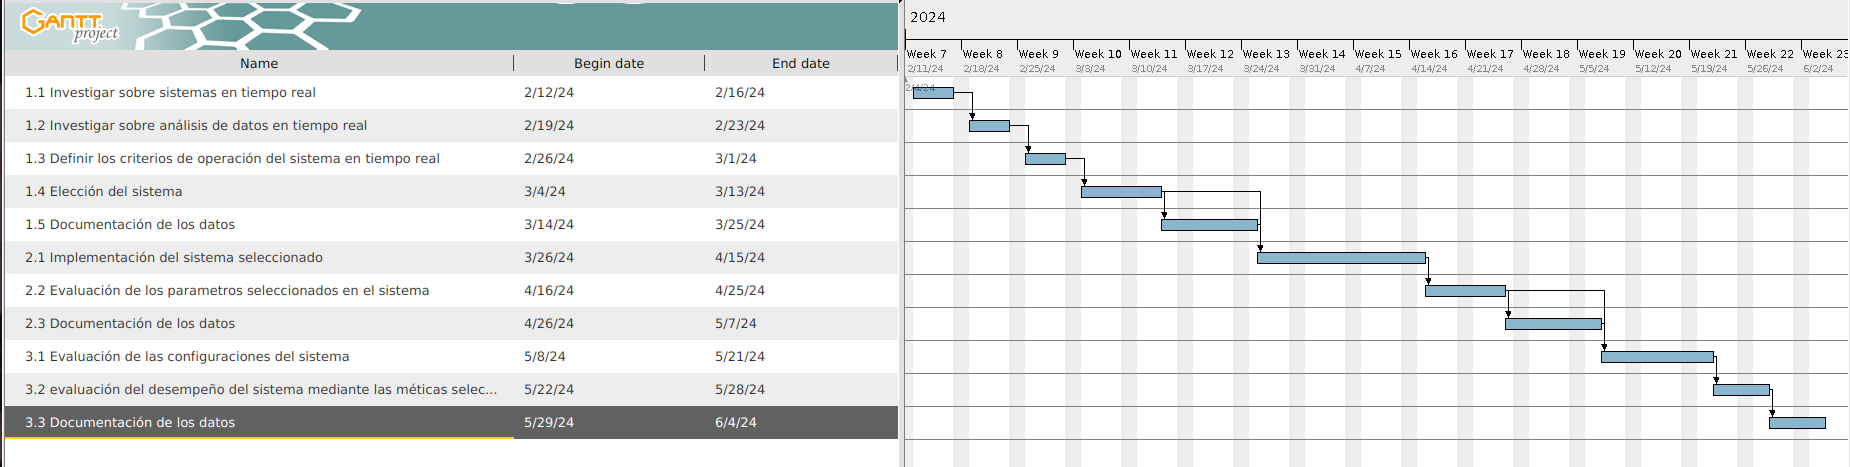
\includegraphics[width=0.8\textwidth]{diagramas/gantt.png}
  \caption{Diagrama de Gantt para el desarrollo del proyecto}
  \label{fig:gantt}
\end{figure}

Para obtener \dots

\begin{figure}[h!]
  \centering
  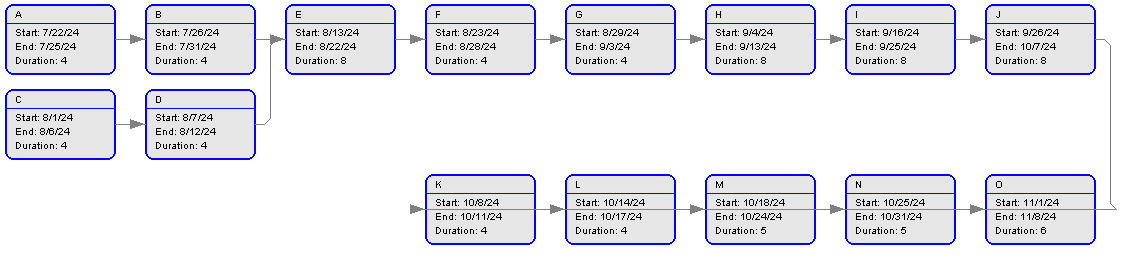
\includegraphics[width=0.8\textwidth]{diagramas/pert.png}
  \caption{Diagrama de PERT para el desarrollo del proyecto}
  \label{fig:pert}
\end{figure}

\subsection{Entregables}

Como se puede observar en el Cuadro se encuentra una lista de los entregables con sus objetivos y fechas de entrega establecidas en el periodo donde se llevara a cabo el trabajo final de graduación.

\begin{table}[h!]
  \caption{Entregables}
  \label{tab:entregables}
  \resizebox{\textwidth}{!}{%
  \begin{tabular}{|l|l|l|}
  \hline
  Objetivo     & Entregable                                                                                      & Fecha de entrega \\ \hline
  Específico 1 & \begin{tabular}[c]{@{}l@{}}Modelo y número de parte de la tarjeta\\ seleccionada.\end{tabular}  &                  \\ \hline
  Específico 2 &
    \begin{tabular}[c]{@{}l@{}}Flujos de trabajo para algoritmos de\\ control, orientación y navegación\\ con hardware en el loop.\end{tabular} &
     \\ \hline
  Específico 3 & \begin{tabular}[c]{@{}l@{}}Resultados obtenidos para el caso de\\ uso seleccionado\end{tabular} &                  \\ \hline
  General 1 &
    \begin{tabular}[c]{@{}l@{}}Repositorio en GitHub con la documentación\\ y programas generados para el funcionamiento\\ de los flujos de trabajo implementados\end{tabular} &
     \\ \hline
  \end{tabular}%
  }
  \end{table}

\section{Uso de recursos}

Para desarrollar el conjunto de flujos de trabajo se hace uso de la siguiente lista de Materiales.

\begin{itemize}
  \item Computadora donde desarrollar y probar los distintos flujos de trabajo.
  \item Tarjeta de desarrollo.
  \item Acceso a internet para llevar a cabo la revisión bibliográfica.
\end{itemize}

\newpage

\section{Presupuesto}

Se realiza la estimación del presupuesto. 


\newpage
\nocite{moghaddam2021guidance}
\nocite{zhang2021guidance}
\nocite{karimi2021guidance}
\nocite{hewing2023enhancing}
\nocite{chai2021review}
\nocite{bitlmal2024guidance}
\nocite{bai2023vision}
\nocite{qinghua2023navigation}
\nocite{wang2022deep}
\nocite{gandhiterminal}
\nocite{Colmenarejo2024}
\nocite{AEM2017}
\nocite{Gutierrez2022}
\nocite{Ortega2021}
\nocite{Colmenarejo2022}
\nocite{TecCR2023_MUSA}
\nocite{TecCR2023_Satelite}
\nocite{Furfaro1997}
\nocite{Bouabdallah2009}
\nocite{Balaram2008}
\nocite{MathWorks2024_ss}
\nocite{MathWorks2024}

\bibliography{bibliografia.bib}
\bibliographystyle{plain}

\end{document}